\documentclass{beamer}

% Tema
\usetheme{CambridgeUS}

% Paquetes
\usepackage[utf8]{inputenc}
\usepackage[spanish]{babel}
\usepackage{graphicx}
\usepackage{amsmath}
\usepackage{physics}
\usepackage{siunitx}

% Configuración de paquetes
\sisetup{
  per-mode = symbol,
  fraction=nice
}

% Título y autor
\title{Del átomo a la industria: \\ cómo la simulación científica transforma la ingeniería}
\author{Felipe Wasaff}
\institute{
  \smallskip
  \begin{tabular}{c}
    Grupo de NanoMateriales \\
    Facultad de Ciencias, Universidad de Chile \\
    \smallskip
    \& \\
    \smallskip
    Wasaff Consulting \\
 \end{tabular}
}
\date{2025}

% Logo adicional
\titlegraphic{
  
\includegraphics[height=1cm]{logo_uchile.jpg}\hspace*{1cm}~
  
\includegraphics[height=1cm]{logo_ust.png}
}

\begin{document}

% Portada
\begin{frame}
  \titlepage
\end{frame}

% Índice
\begin{frame}{Contenido}
  \tableofcontents
\end{frame}

\section{Introducción}

\begin{frame}{¿Por qué estoy aquí?}
  \begin{itemize}
    \item Soy físico e ingeniero en automatización
    \item Trabajo en simulaciones científicas y desarrollo de tecnología
    \item Hoy mostraré cómo un experimento teórico puede impactar:
    \begin{itemize}
      \item Construcción (materiales, estructuras)
      \item Automatización (control de procesos)
      \item Electricidad (conductividad, pérdidas energéticas)
    \end{itemize}
  \end{itemize}
\end{frame}

\begin{frame}{Pregunta fundamental}
  \begin{block}{¿Cómo predecir el comportamiento de la materia desde los átomos hasta los sistemas macroscópicos?}
  \end{block}
  \begin{columns}
    \column{0.5\textwidth}
    \centering
    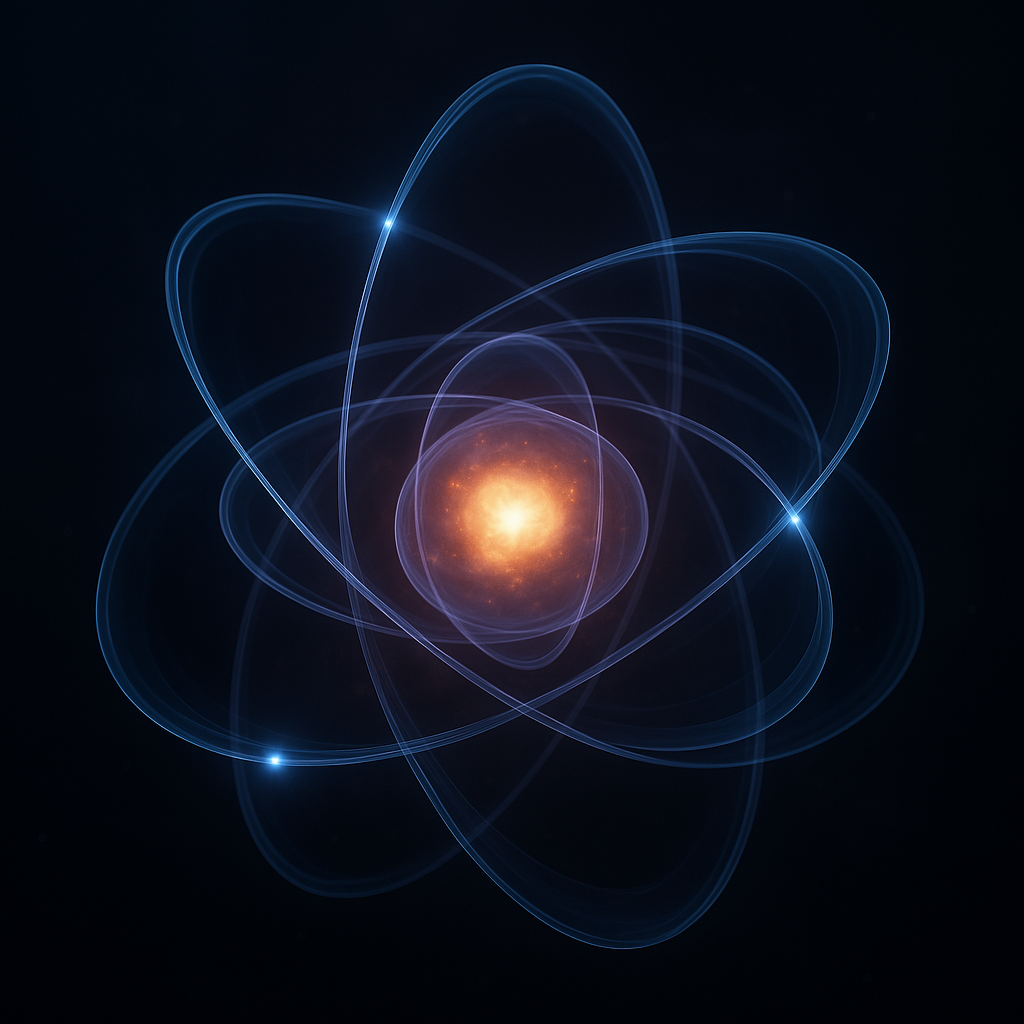
\includegraphics[width=0.8\linewidth]{atom.png}\\
    {\small Escala atómica (\SI{e-10}{\meter})}
    
    \column{0.5\textwidth}
    \centering
    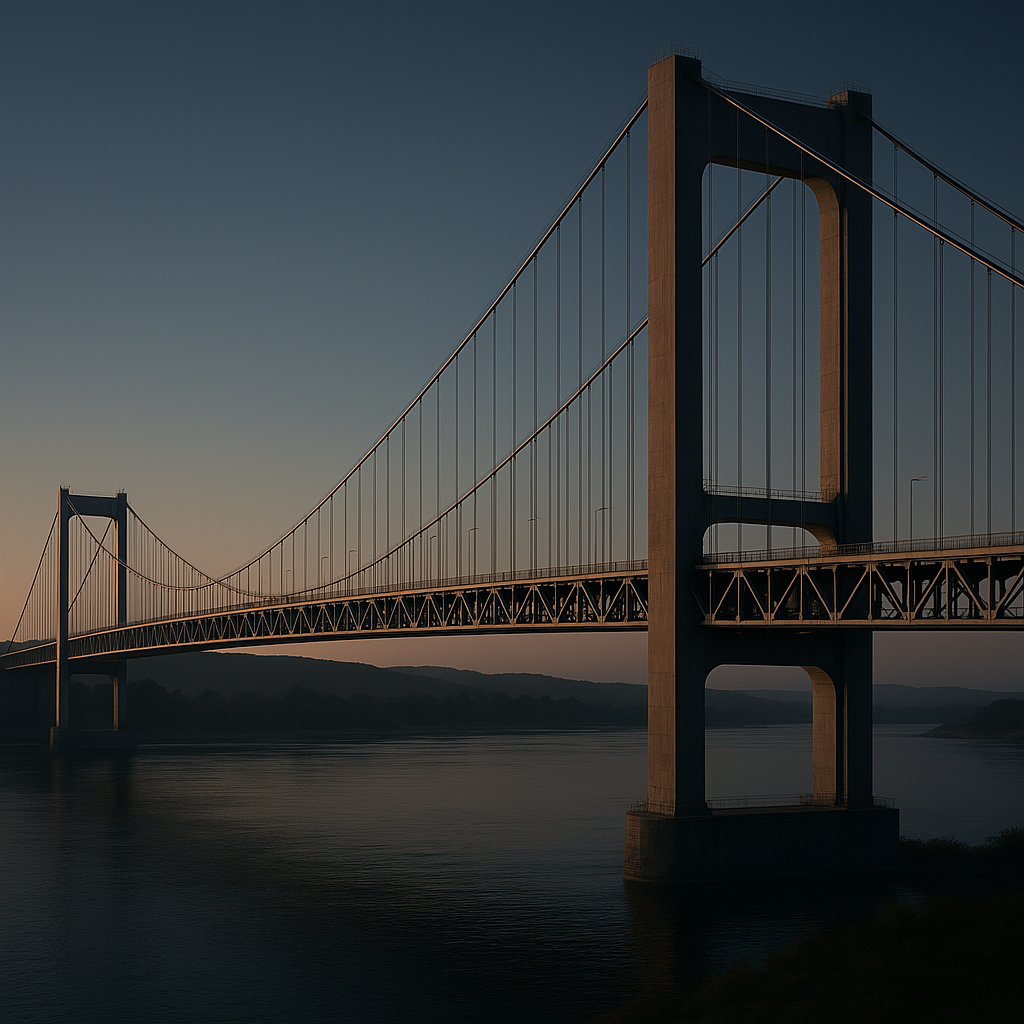
\includegraphics[width=0.8\linewidth]{bridge.png}\\
    {\small Escala macroscópica (\SI{e1}{\meter})}
  \end{columns}
\end{frame}

\section{Fundamentos teóricos}

\begin{frame}{Dinámica Molecular: Base matemática}
  \begin{block}{Ecuaciones de movimiento}
    \[
    m_i \dv[2]{\vec{r}_i}{t} = \vec{F}_i = -\nabla_i V(\vec{r}_1, \dots, \vec{r}_N)
    \]
    donde:
    \begin{itemize}
      \item $m_i$: masa del átomo $i$
      \item $\vec{r}_i$: posición del átomo $i$
      \item $V$: potencial interatómico
    \end{itemize}
  \end{block}
  
  \begin{block}{Potencial de Lennard-Jones (para argón)}
    \[
    V(r_{ij}) = 4\epsilon \left[ \left(\frac{\sigma}{r_{ij}}\right)^{12} - \left(\frac{\sigma}{r_{ij}}\right)^6 \right]
    \]
    $\epsilon=\SI{0.0104}{\electronvolt}$, $\sigma=\SI{3.4}{\angstrom}$
  \end{block}
\end{frame}

\begin{frame}{Algoritmo de Verlet}
  Método numérico para integrar las ecuaciones de movimiento:
  \[
  \vec{r}(t + \Delta t) = 2\vec{r}(t) - \vec{r}(t - \Delta t) + \frac{\vec{F}(t)}{m} \Delta t^2 + \mathcal{O}(\Delta t^4)
  \]
  \begin{itemize}
    \item Precisión de cuarto orden
    \item Conserva energía en sistemas cerrados
    \item Paso temporal típico: \SI{1}{\femto\second} (\SI{e-15}{\second})
  \end{itemize}
\end{frame}

\section{Simulación científica}

\begin{frame}{Software libre para simulaciones}
  \begin{columns}
    \column{0.5\textwidth}
    \textbf{Dinámica Molecular:}
    \begin{itemize}
      \item LAMMPS (este trabajo)
      \item GROMACS
      \item NAMD
    \end{itemize}
    
    \textbf{Visualización:}
    \begin{itemize}
      \item OVITO
      \item VMD
      \item ParaView
    \end{itemize}
    
    \column{0.5\textwidth}
    \textbf{Análisis de datos:}
    \begin{itemize}
      \item Python (NumPy, SciPy)
      \item Jupyter Notebooks
      \item R
    \end{itemize}
    
    \textbf{Machine Learning:}
    \begin{itemize}
      \item Scikit-learn
      \item TensorFlow/PyTorch
    \end{itemize}
  \end{columns}
\end{frame}

\begin{frame}{Flujo de trabajo típico}
  \centering
  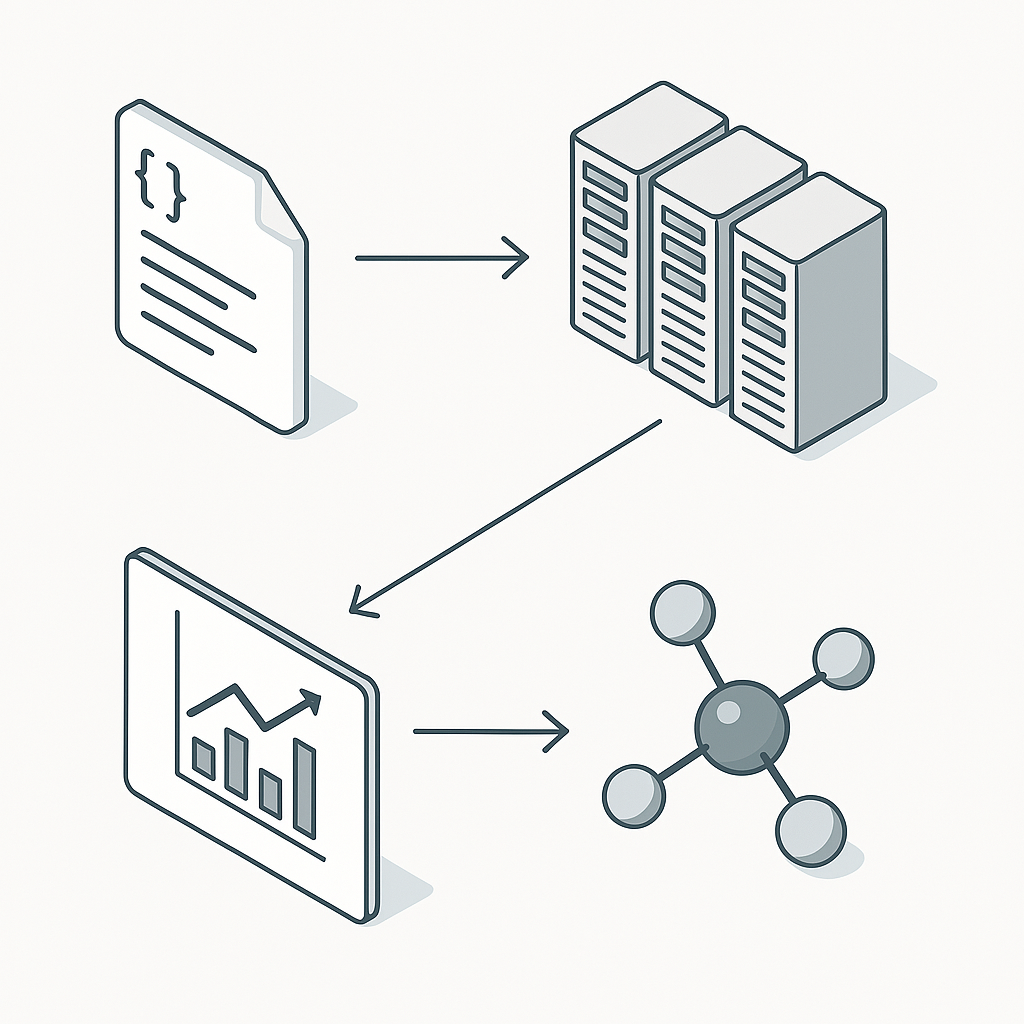
\includegraphics[width=0.7\linewidth]{workflow.png}
  
  \begin{enumerate}
    \item Definición del sistema (LAMMPS input script)
    \item Simulación (HPC/cluster)
    \item Análisis (Python)
    \item Visualización (OVITO/ParaView)
  \end{enumerate}
\end{frame}

\section{Caso práctico: Colisión de un clúster de argón}

\begin{frame}{Configuración de la simulación}
  \begin{columns}
    \column{0.6\textwidth}
    \begin{itemize}
      \item 500 átomos de Argon (cluster esférico)
      \item Superficie rígida de Ni (100)
      \item Velocidad inicial: \SI{500}{\meter\per\second}
      \item Tiempo total: \SI{20}{\pico\second}
      \item Condiciones:
      \begin{itemize}
        \item NVE (sistema cerrado)
        \item Termostato Langevin
      \end{itemize}
    \end{itemize}
    
    \column{0.4\textwidth}
    \centering
    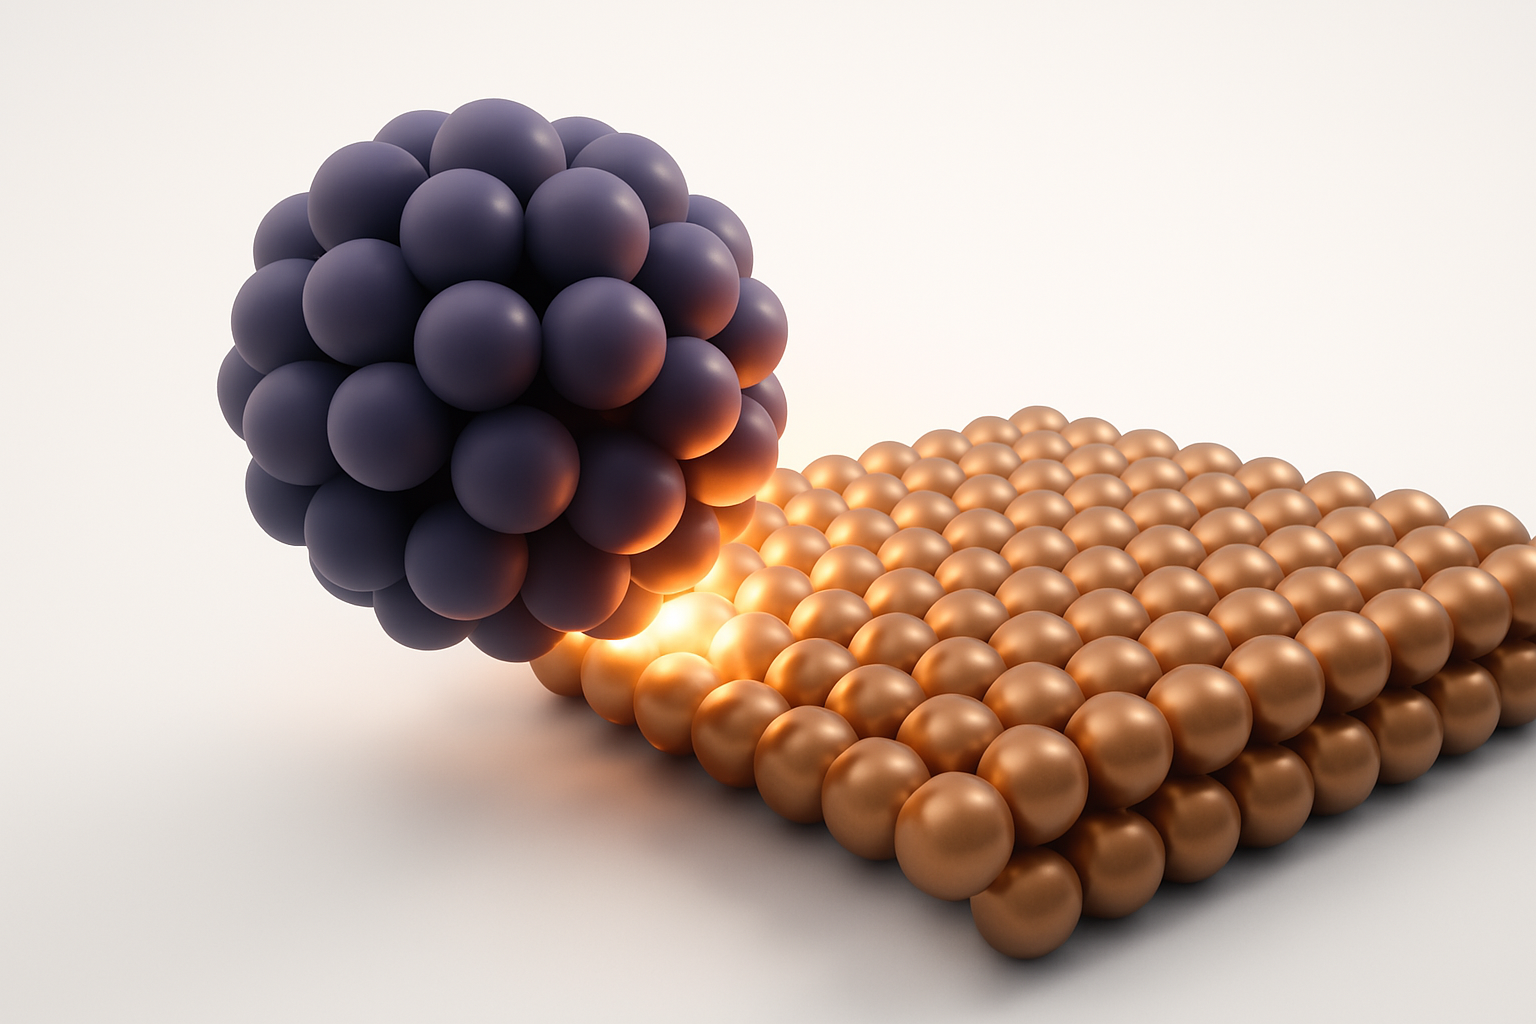
\includegraphics[width=\linewidth]{sim_setup.png}
  \end{columns}
\end{frame}

\begin{frame}{Resultados clave}
  \begin{columns}
    \column{0.5\textwidth}
    \centering
    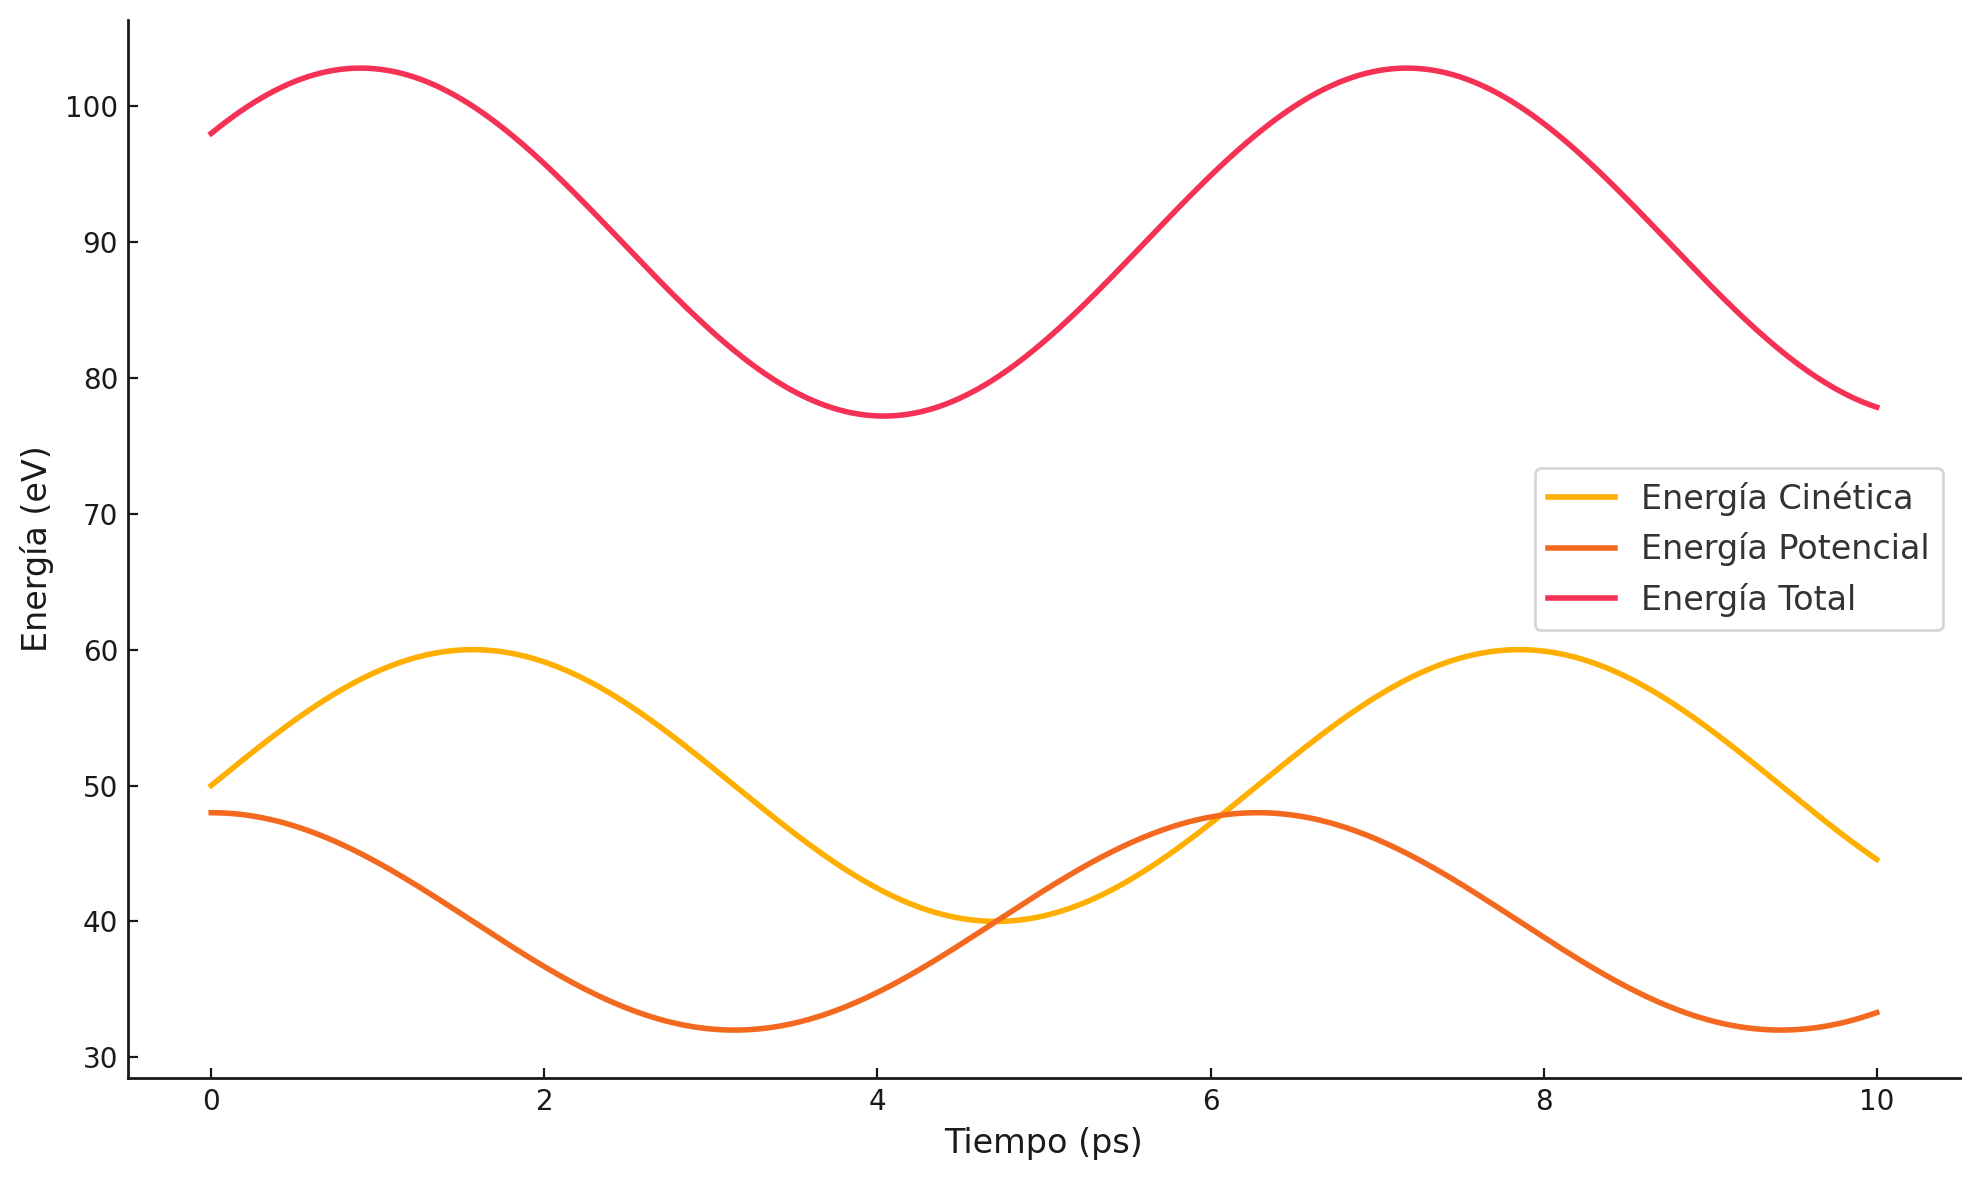
\includegraphics[width=\linewidth]{energy_plot.png}\\
    \small Evolución energética
    
    \column{0.5\textwidth}
    \centering
    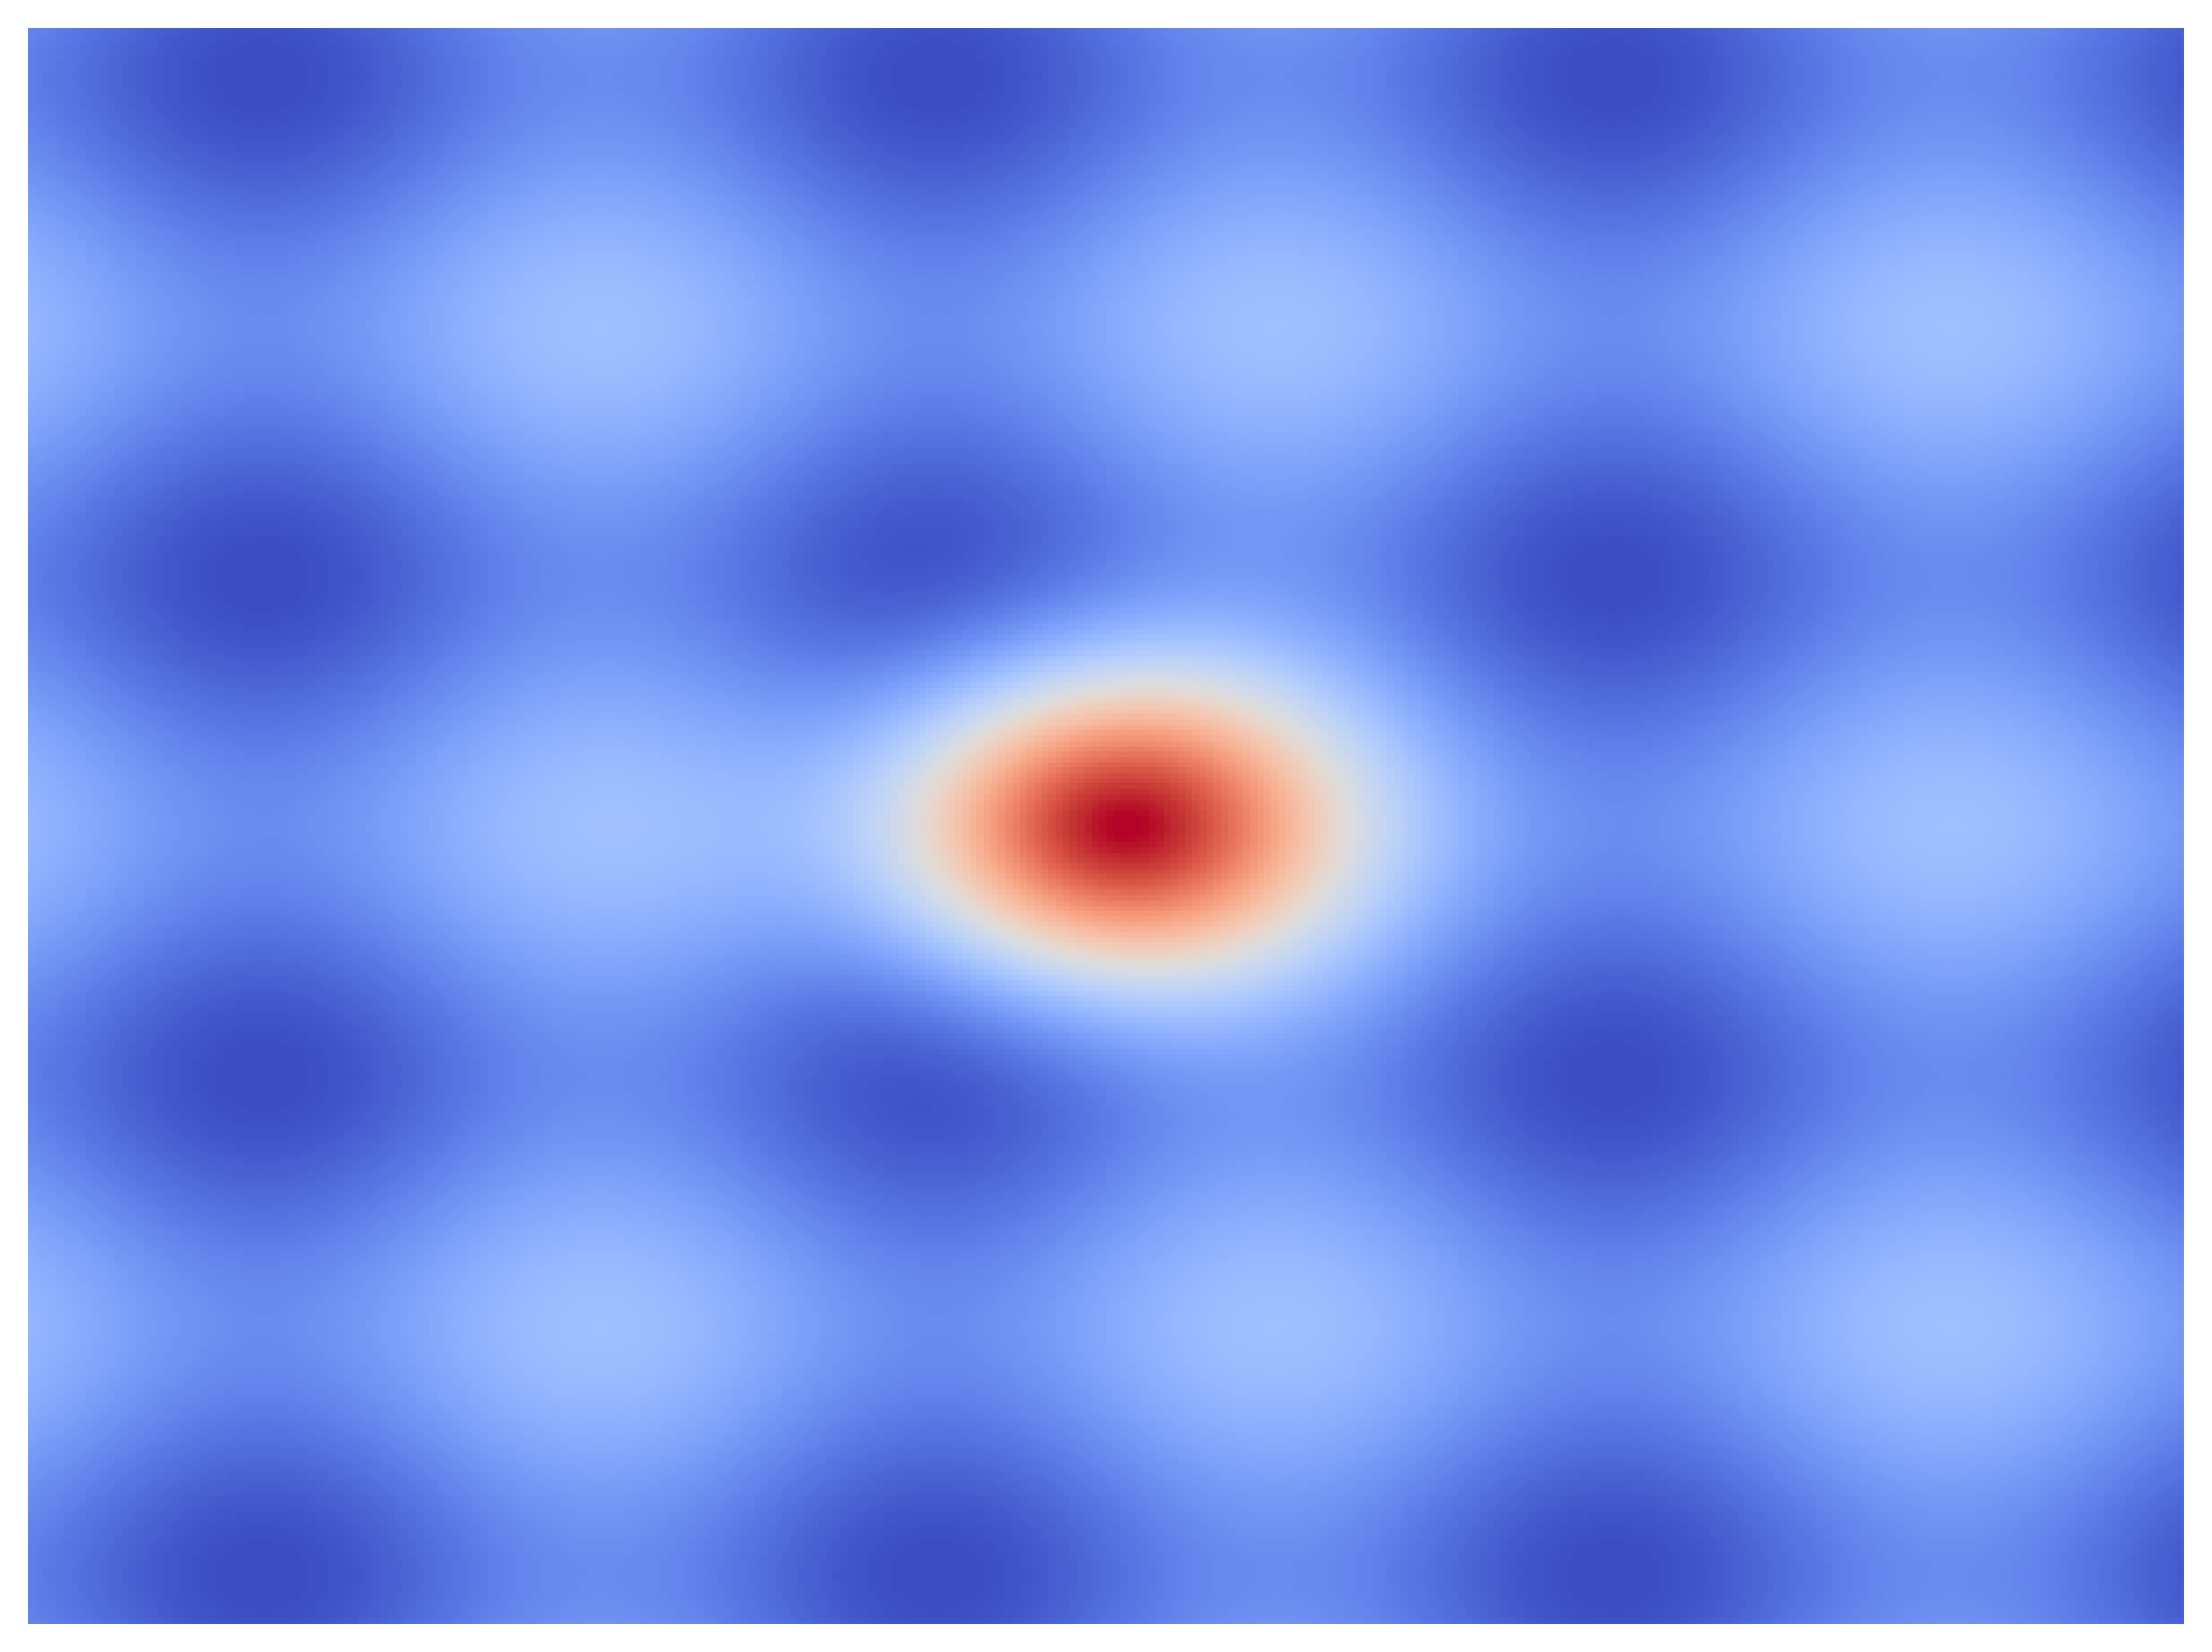
\includegraphics[width=\linewidth]{temperature_plot.png}\\
    \small Distribución de temperatura
  \end{columns}
  
  \vspace{5mm}
  \begin{equation*}
    T(t) = \frac{2}{3N k_B} \langle E_k \rangle
  \end{equation*}
\end{frame}

\begin{frame}{Análisis de disipación energética}
  \begin{block}{Modelo teórico}
    \[
    \frac{dE}{dt} = -\alpha (T_{cluster} - T_{surface}) - \beta \left(\frac{dE}{dx}\right)_{vib}
    \]
    donde:
    \begin{itemize}
      \item $\alpha$: coeficiente de transferencia térmica
      \item $\beta$: factor de amortiguamiento vibracional
    \end{itemize}
  \end{block}
  
  \begin{block}{Resultados de simulación}
    \begin{itemize}
      \item 60\% de energía disipada como calor
      \item 30\% convertida en vibraciones de red
      \item 10\% permanece como energía cinética
    \end{itemize}
  \end{block}
\end{frame}

\section{Modelado predictivo}

\begin{frame}{Machine Learning aplicado}
  \begin{block}{Objetivo}
    Predecir disipación energética sin simulaciones completas
  \end{block}
  
  \begin{columns}
    \column{0.6\textwidth}
    \textbf{Datos de entrenamiento:}
    \begin{itemize}
      \item 500 simulaciones variando:
      \begin{itemize}
        \item Velocidad (100-1000 m/s)
        \item Tamaño del cluster (50-1000 átomos)
        \item Temperatura superficie (100-500 K)
      \end{itemize}
      \item Features: parámetros iniciales
      \item Targets: resultados finales
    \end{itemize}
    
    \column{0.4\textwidth}
    \centering
    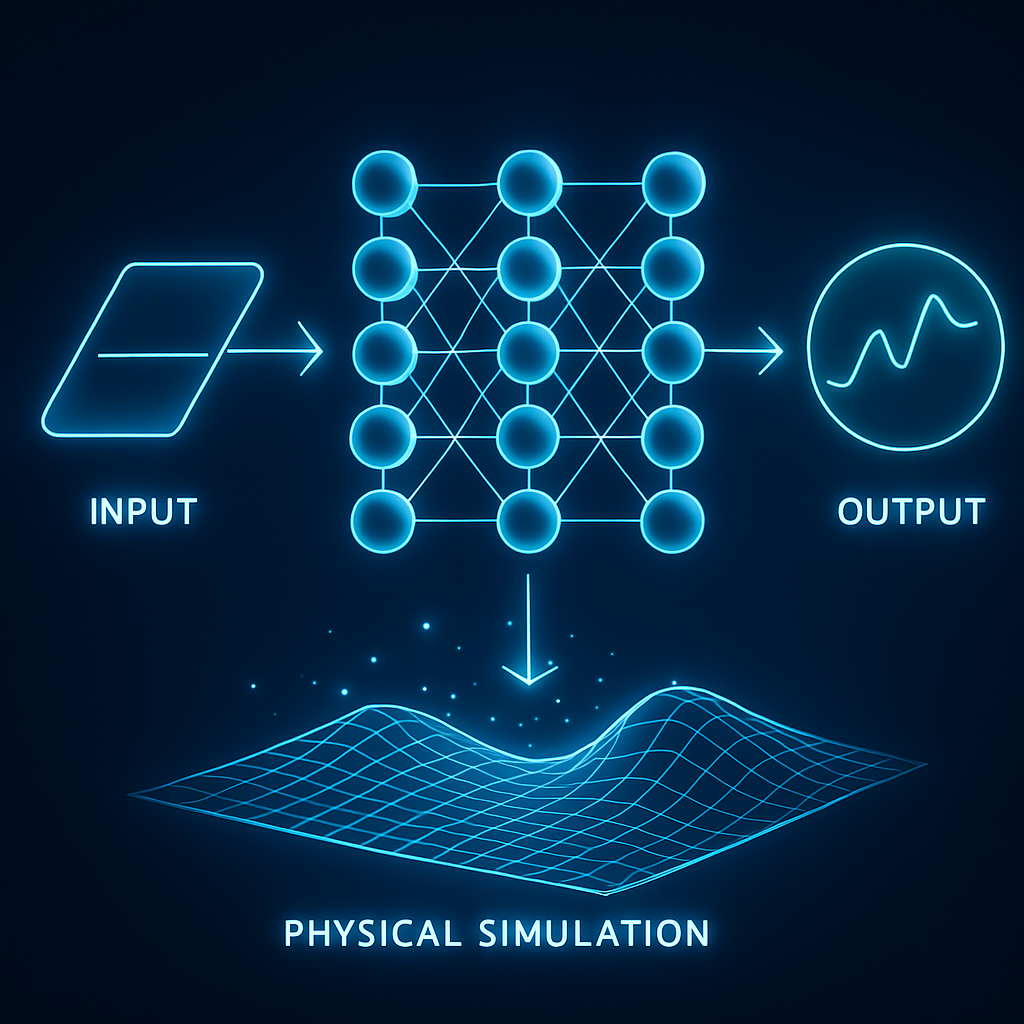
\includegraphics[width=\linewidth]{ml_model.png}
  \end{columns}
\end{frame}

\begin{frame}{Arquitectura del modelo}
  \begin{columns}
    \column{0.5\textwidth}
    \textbf{Red Neuronal:}
    \begin{itemize}
      \item 3 capas ocultas (64, 32, 16 neuronas)
      \item Función de activación ReLU
      \item Optimizador Adam
      \item Loss: MSE
    \end{itemize}
    
    \textbf{Rendimiento:}
    \begin{itemize}
      \item R$^2$ = 0.92 (train)
      \item R$^2$ = 0.89 (test)
      \item Tiempo predicción: \SI{10}{\milli\second}
    \end{itemize}
    
    \column{0.5\textwidth}
    \centering
    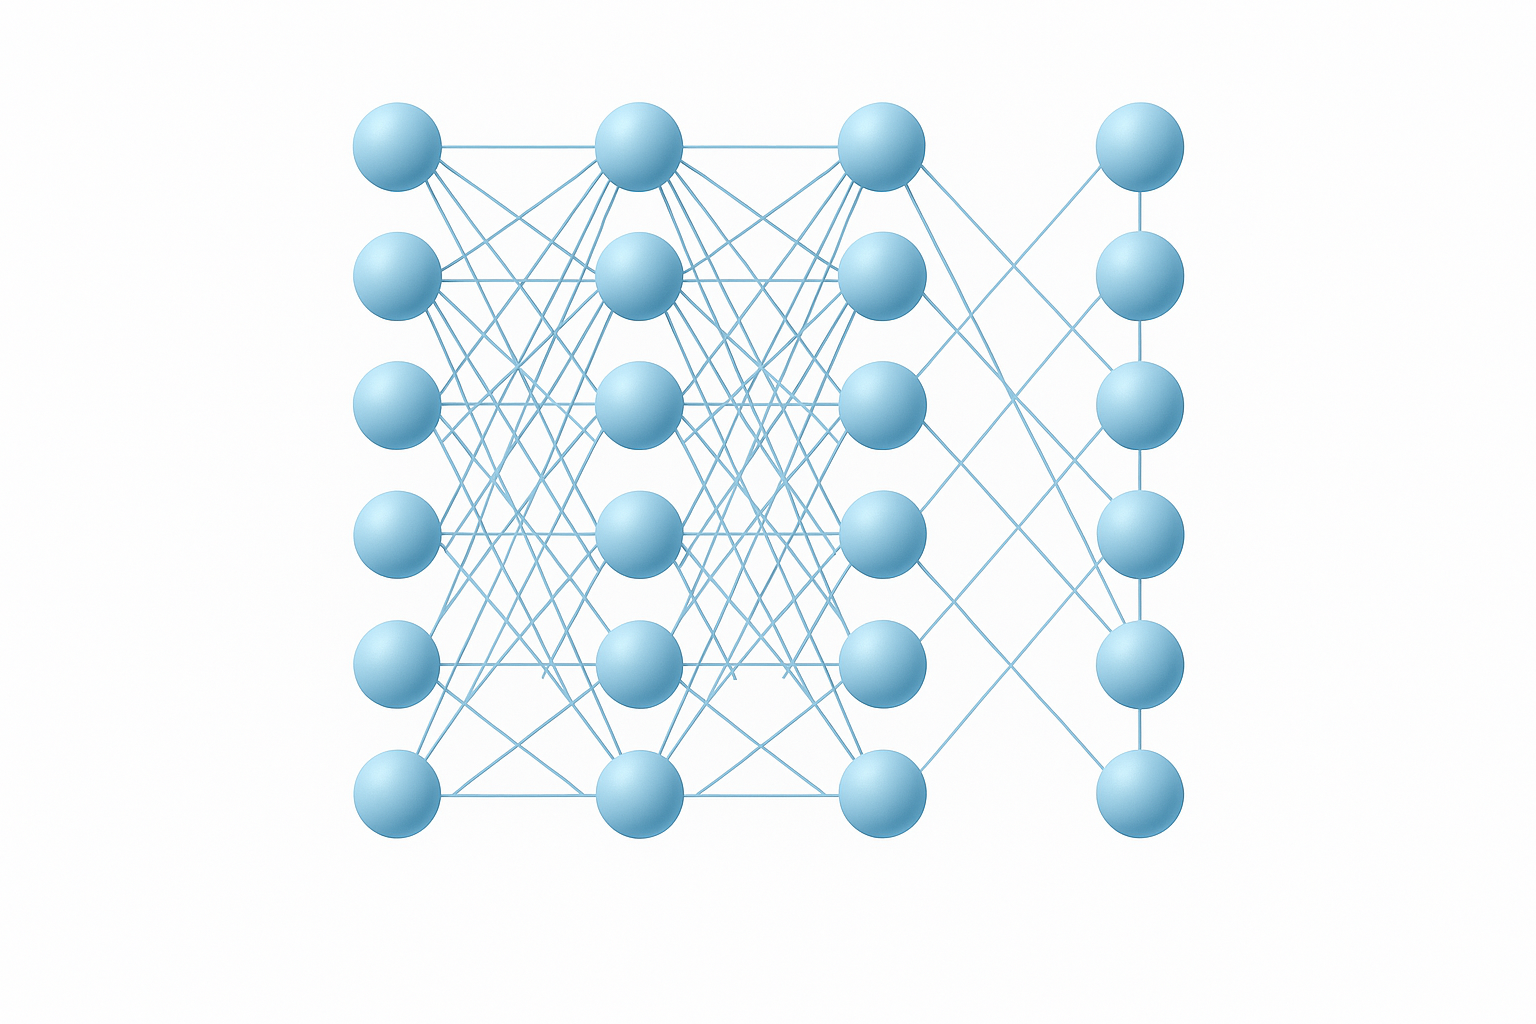
\includegraphics[width=\linewidth]{nn_architecture.png}
  \end{columns}
\end{frame}

\section{Aplicaciones industriales}

\begin{frame}{Transferencia tecnológica}
  \begin{columns}
    \column{0.5\textwidth}
    \textbf{Construcción:}
    \begin{itemize}
      \item Diseño de materiales absorbentes de impacto
      \item Optimización de aislantes térmicos
      \item Modelado de fatiga en metales
    \end{itemize}
    
    \textbf{Electricidad:}
    \begin{itemize}
      \item Disipación térmica en componentes
      \item Materiales para contactos eléctricos
    \end{itemize}
    
    \column{0.5\textwidth}
    \textbf{Automatización:}
    \begin{itemize}
      \item Control de procesos térmicos
      \item Predicción de fallas en maquinaria
      \item Optimización de robots colaborativos
    \end{itemize}
    
    \textbf{Nanotecnología:}
    \begin{itemize}
      \item Diseño de nanocompuestos
      \item Sistemas de liberación controlada
    \end{itemize}
  \end{columns}
\end{frame}

\begin{frame}{Ejemplo concreto: Aislante térmico}
  \begin{columns}
    \column{0.6\textwidth}
    \begin{itemize}
      \item Material poroso inspirado en estructura de clusters
      \item Simulación de transferencia térmica:
      \[
      \kappa_{eff} = \frac{1}{3} C v \lambda
      \]
      donde:
      \begin{itemize}
        \item $C$: capacidad calorífica
        \item $v$: velocidad fonónica
        \item $\lambda$: camino libre medio
      \end{itemize}
      \item Resultado: 40\% mejor aislamiento
    \end{itemize}
    
    \column{0.4\textwidth}
    \centering
    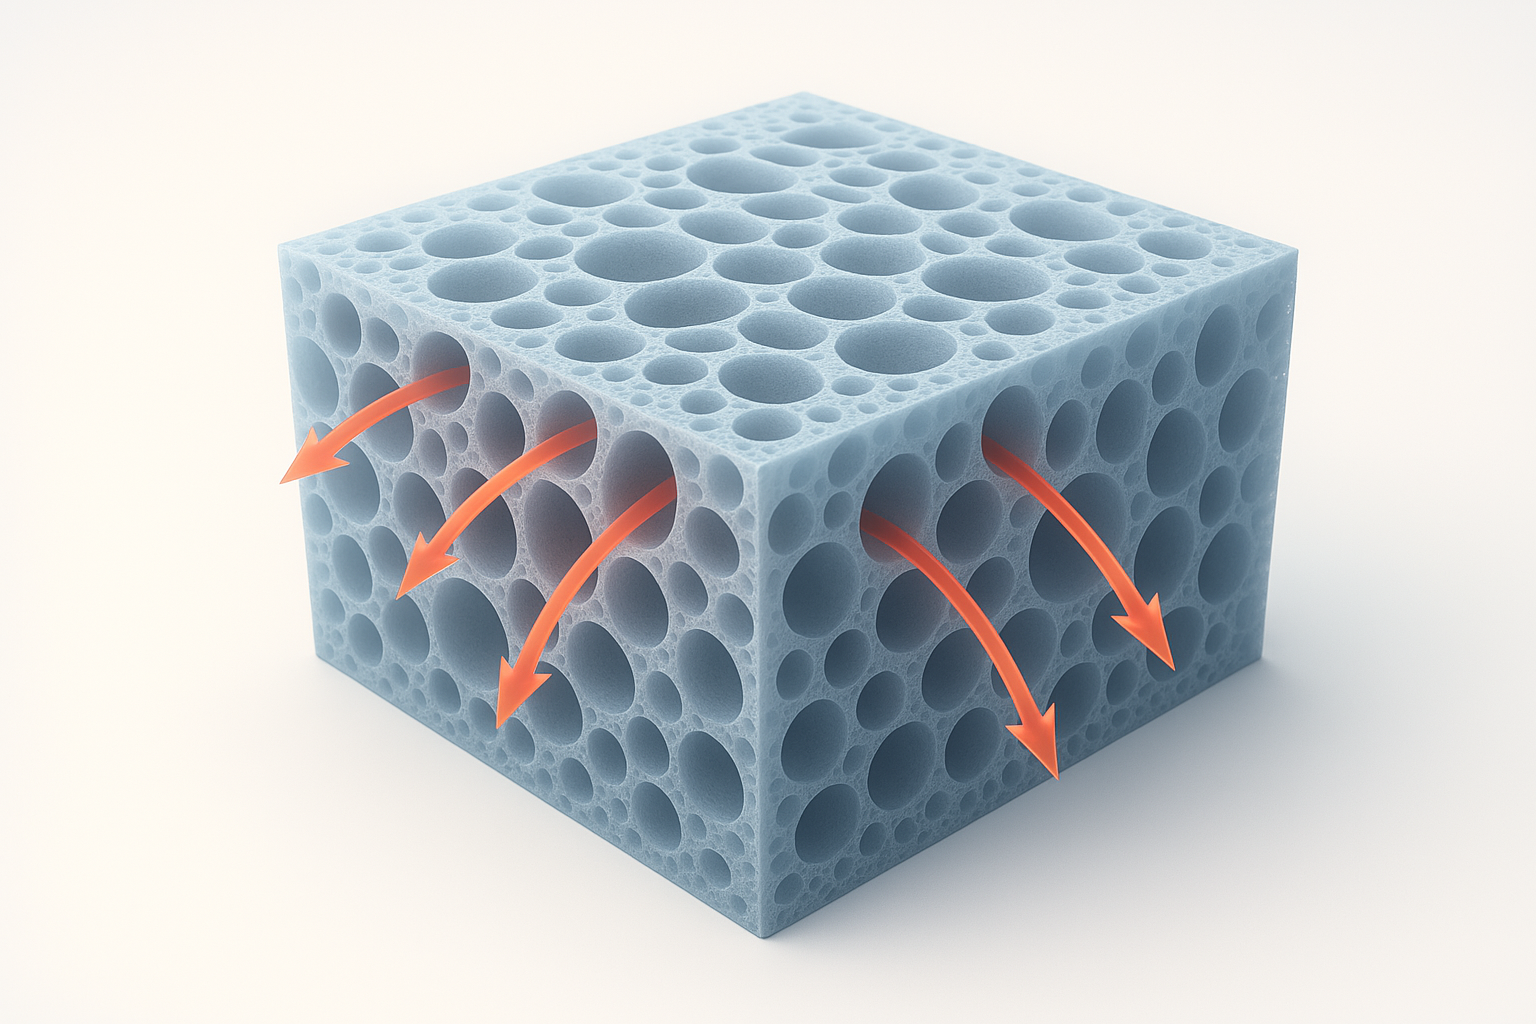
\includegraphics[width=\linewidth]{insulator.png}
  \end{columns}
\end{frame}

\section{Conclusión}

\begin{frame}{El futuro de la ingeniería computacional}
  \begin{itemize}
    \item \textbf{Multiescala}: De átomos a sistemas completos
    \item \textbf{Interdisciplina}: Física + Ingeniería + Ciencia de Datos
    \item \textbf{Open Science}: Software libre y reproducible
  \end{itemize}
  
  \begin{block}{Oportunidad para Chile}
    Podemos ser líderes en ingeniería computacional aplicada a:
    \begin{itemize}
      \item Minería (desgaste de materiales)
      \item Energía (almacenamiento, conversión)
      \item Construcción (materiales inteligentes)
    \end{itemize}
  \end{block}
\end{frame}

\begin{frame}{Invitación a colaborar}
  \centering
  \textbf{\Large ¿Preguntas? Ideas? Proyectos?}
  
  \vspace{5mm}
  \texttt{felipe@wasaffconsulting.com}
  
  \vspace{5mm}
  \small Repositorio con ejemplos: \url{https://github.com/example/MD-demo}
  
  \vspace{5mm}
  
\includegraphics[width=0.2\linewidth]{qr-code.png}
\end{frame}

\end{document}
